% Asal-usul (tidak pernah dicetak): lihat sources/outline_sources.md (Tahun 1: lempeng kaku pada
% bola, kutub dan vektor Euler; kecepatan relatif; titik tiga; rotasi berhingga; skala waktu anomali
% magnetik; geodesi satelit). Peta dan kurva dari figdata/bachelor-1/euler_velocities.py,
% south_atlantic_fit.py dan gpts_stripes.py; nilai soal latihan dan soal dihitung dalam kalkulator
% skrap Buku 3 calc/ch12.py.
\chapter{Kinematika lempeng pada bola}\label{ch:b1:plate-kinematics}

Dua stasiun penentuan posisi satelit telah merekam posisinya setiap hari selama lebih dari seperempat abad: satu di Reykjavik, di barat Islandia, yang lain di dekat Stavanger, di pantai barat Norwegia. Garis lurus di antara keduanya, sepanjang \qty{1546}{km}, bertambah \qty{17.5}{mm} setiap tahun, hampir dua sentimeter. Tidak ada yang tampak di permukaan tanah, namun dasar Atlantik Utara di antara kedua stasiun mencatat pelebaran yang sama selama jutaan tahun: lava yang meletus di Punggungan Atlantik Tengah mengambil arah medan magnet Bumi ketika mendingin, dan medan itu telah berbalik arah berkali-kali, sehingga dasar samudra memuat catatan bergaris tentang pertumbuhannya sendiri. Bab ini mengubah lempeng-lempeng dari tahun-tahun sekolah menjadi tudung kaku di atas bola, menggambarkan gerakannya dengan geometri rotasi, dan menunjukkan bagaimana catatan geologi dan satelit mengukur gerakan yang sama.
% ledger: ngl:reyk, ngl:stas (chord lengthening computed in calc/ch12.py)

\begin{recall}
Pada bola, \omterm{def:b1:spherical-astronomy:spherical-triangle}{lingkaran besar} adalah perpotongan dengan bidang yang melalui pusat, \omterm{def:b1:spherical-astronomy:spherical-triangle}{lingkaran kecil} dengan bidang lain apa pun; kaidah kosinus memberikan jarak sudut antara dua titik dari \omterm{def:b1:spherical-astronomy:geographic}{lintang} dan \omterm{def:b1:spherical-astronomy:geographic}{bujurnya}, dan \omterm{def:b1:spherical-astronomy:horizontal}{azimut} suatu arah dihitung dari utara melalui timur (\cref{ch:b1:spherical-astronomy}). Benda tegar yang berputar terhadap sumbu tetap memiliki kecepatan sudut (fisika). \omterm{def:b1:layered-earth:lithosphere}{Litosfer} pecah menjadi lempeng-lempeng yang bergerak relatif satu sama lain beberapa sentimeter per tahun, dan dasar samudra memuat garis-garis magnetik yang mencatat pembalikan medan magnet Bumi (Buku 2, kelas 11).
\end{recall}

\section{Lempeng kaku pada bola}

Sebuah lempeng menutupi sebagian besar bola: lempeng Eurasia membentang dari tengah Atlantik hingga Siberia timur. Geraknya tidak dapat digambarkan dengan kecepatan, seperti gerak mobil; ia harus digambarkan dengan rotasi.

\begin{definition}[Lempeng kaku]\label{def:b1:plate-kinematics:rigid-plate}
Sebuah \emph{lempeng kaku}\index{lempeng kaku} adalah suatu wilayah \omterm{def:b1:layered-earth:lithosphere}{litosfer} yang bagian dalamnya tidak berdeformasi secara terukur: jarak antara dua titik mana pun di dalamnya tetap konstan. Gerak relatif dua lempeng diserap di sepanjang batas bersama mereka, sebuah zona sempit patahan, gempa dan gunung api.
\end{definition}

Tidak ada lempeng yang benar-benar kaku: batasnya adalah zona yang lebarnya puluhan hingga ratusan kilometer, dan bagian dalamnya berdeformasi perlahan. Hipotesisnya adalah bahwa penyimpangan ini kecil dibanding gerak relatif; hipotesis itu diuji oleh konsistensi setiap hasil dalam bab ini.

\omterm{def:b1:plate-kinematics:rigid-plate}{Lempeng kaku} di permukaan bola bergerak tanpa mengubah jarak antara dua titik mana pun di dalamnya, dan pusat Bumi tidak bergerak. Gerak semacam itu digambarkan oleh matriks $3\times3$ $R$ yang mempertahankan panjang, sebuah matriks \emph{ortogonal} ($R^{\mathsf T}R = I$), dan yang mempertahankan orientasi ruang, sehingga $\det R = 1$: titik pada vektor posisi $\vec r$ pergi ke $R\vec r$.

\begin{theorem}[Teorema rotasi Euler]\label{thm:b1:plate-kinematics:euler}
Setiap perpindahan \omterm{def:b1:plate-kinematics:rigid-plate}{lempeng kaku} di atas bola adalah rotasi terhadap sumbu yang melalui pusat Bumi: ada vektor satuan $\vec n$ dengan $R\vec n = \vec n$, dan lempeng berputar terhadap $\vec n$ dengan suatu sudut.
\end{theorem}

\begin{proof}
Kita tunjukkan bahwa $1$ adalah nilai eigen $R$, yaitu $\det(R - I) = 0$. Karena $R R^{\mathsf T} = I$, kita memiliki $R - I = R(I - R^{\mathsf T})$, sehingga
\[
  \det(R - I) = \det R\,\det\bigl((I - R)^{\mathsf T}\bigr) = \det(I - R),
\]
menggunakan $\det R = 1$ dan fakta bahwa suatu matriks dan transposenya memiliki determinan yang sama. Untuk matriks $3\times3$,
$\det(I - R) = (-1)^3\det(R - I) = -\det(R - I)$. Jadi $\det(R - I) =
-\det(R - I)$, yang nol. Sebuah vektor satuan $\vec n$ dengan $R\vec n = \vec n$ karena itu ada: kedua titik tempat garis melalui pusat sepanjang $\vec n$ memotong permukaan tidak bergerak. Pada bidang tegak lurus $\vec n$, $R$ mempertahankan panjang dan orientasi: ia memutar bidang itu dengan suatu sudut, sehingga ia memutar seluruh bola terhadap $\vec n$.
\end{proof}

Selama interval waktu yang cukup pendek agar gerak tidak berubah, rotasi berlangsung dengan laju tetap, dan gerak satu lempeng relatif terhadap lempeng lain adalah kecepatan sudut terhadap sumbu tetap.

\begin{definition}[Kutub Euler; vektor Euler]\label{def:b1:plate-kinematics:euler-pole}
Gerak lempeng B relatif terhadap lempeng A adalah rotasi terhadap sumbu yang melalui pusat Bumi. \emph{Kutub Euler}\index{kutub Euler} pasangan itu adalah titik tempat sumbu ini memotong permukaan, dipilih sehingga rotasinya berlawanan arah jarum jam bila dilihat dari atasnya; titik antipodalnya adalah kutub yang berlawanan. \emph{Vektor Euler}\index{vektor Euler}
$\vec\omega_{BA}$ adalah kecepatan sudut B relatif terhadap A: ia menunjuk dari pusat Bumi ke kutub Euler, dan panjangnya $\omega$ adalah laju rotasinya.
\end{definition}

\omterm{def:b1:plate-kinematics:euler-pole}{Vektor Euler} diberikan oleh \omterm{def:b1:spherical-astronomy:geographic}{lintang} dan \omterm{def:b1:spherical-astronomy:geographic}{bujur} kutubnya serta lajunya, biasanya dalam derajat per juta tahun. Gerak lempeng Eurasia relatif terhadap lempeng Amerika Utara, dirata-ratakan selama \qty{3.16}{Ma} terakhir dari 453 laju penyebaran yang diukur pada punggungan di antara keduanya, memiliki kutubnya pada \ang{61.8}\,U, \ang{139.6}\,T, di Siberia timur, dan lajunya \qty{0.210}{\degree\per\Ma}. Dalam radian per tahun,
\[
  \omega = \frac{0.210\times\pi/180}{\num{e6}} = \qty{3.665e-9}{rad.yr^{-1}},
\]
satu putaran penuh dalam \qty{1714}{\Ma}.
% ledger: morvel:eu-na, morvel:summary

\section{Kecepatan relatif}

\begin{theorem}[Kecepatan pada lempeng yang berputar]\label{thm:b1:plate-kinematics:velocity}
Jika lempeng B berputar relatif terhadap lempeng A dengan \omterm{def:b1:plate-kinematics:euler-pole}{vektor Euler} $\vec\omega$, sebuah titik pada B di vektor posisi $\vec r$ (dari pusat Bumi) bergerak relatif terhadap A dengan kecepatan
\[
  \vec v = \vec\omega\times\vec r .
\]
\end{theorem}

\begin{proof}
Misalkan $\Delta$ sudut antara $\vec\omega$ dan $\vec r$. Saat B berputar, titik itu melukiskan lingkaran terhadap sumbu, berjari-jari $R\sin\Delta$,
dengan $R$ jari-jari Bumi; pada laju sudut $\omega$, kelajuannya adalah
$\omega R\sin\Delta$. Kecepatannya tegak lurus pada lingkaran itu, sehingga tegak lurus
baik terhadap sumbu maupun terhadap jari-jari $\vec r$, dan karena rotasinya berlawanan arah jarum jam terhadap $\vec\omega$, arahnya adalah arah $\vec\omega\times\vec r$.
Vektor $\vec\omega\times\vec r$ memiliki tepat arah dan sisi ini serta panjang $\omega R\sin\Delta$.
\end{proof}

Sudut $\Delta$ adalah jarak sudut antara \omterm{def:b1:plate-kinematics:euler-pole}{kutub Euler} dan titik itu, yang dapat diberikan oleh kaidah kosinus dari \omterm{def:b1:spherical-astronomy:geographic}{lintang} dan \omterm{def:b1:spherical-astronomy:geographic}{bujur}.

\begin{proposition}[Kelajuan dan arah gerak relatif]\label{prop:b1:plate-kinematics:speed}
Misalkan \omterm{def:b1:plate-kinematics:euler-pole}{kutub Euler} berada pada \omterm{def:b1:spherical-astronomy:geographic}{lintang} $\varphi_p$ dan \omterm{def:b1:spherical-astronomy:geographic}{bujur} $\lambda_p$, dan titik pada $\varphi$ dan $\lambda$. Maka
\begin{enumerate}
  \item jarak sudut $\Delta$ dari kutub ke titik memenuhi
        $\cos\Delta = \sin\varphi_p\sin\varphi + \cos\varphi_p\cos\varphi
        \cos(\lambda - \lambda_p)$;
  \item kelajuan relatif adalah $v = \omega R\sin\Delta$: nol di kutub,
        terbesar, $\omega R$, pada \omterm{def:b1:spherical-astronomy:spherical-triangle}{lingkaran besar} \ang{90} darinya;
  \item arah gerak tegak lurus terhadap \omterm{def:b1:spherical-astronomy:spherical-triangle}{lingkaran besar} yang menghubungkan titik dengan kutub: \omterm{def:b1:spherical-astronomy:horizontal}{azimutnya} adalah \omterm{def:b1:spherical-astronomy:horizontal}{azimut} kutub, dilihat dari titik, ditambah \ang{90}.
\end{enumerate}
\end{proposition}

\begin{proof}
(1) adalah kaidah kosinus pada \omterm{def:b1:spherical-astronomy:spherical-triangle}{segitiga bola} yang dibentuk oleh kutub utara geografis, \omterm{def:b1:plate-kinematics:euler-pole}{kutub Euler} dan titik itu, yang sisi-sisinya dari kutub utara adalah
$\ang{90} - \varphi_p$ dan $\ang{90} - \varphi$, dengan sudut $\lambda - \lambda_p$ di antaranya. (2) mengikuti dari teorema. (3) Kecepatannya tegak lurus terhadap $\vec\omega$ dan terhadap $\vec r$, sehingga tegak lurus terhadap bidang yang
memuatnya, yaitu bidang \omterm{def:b1:spherical-astronomy:spherical-triangle}{lingkaran besar} yang melalui titik dan kutub. Pada bidang horizontal di titik itu, ia karena itu tegak lurus terhadap arah kutub; rotasinya berlawanan arah jarum jam bila dilihat dari atas kutub, sehingga titik bergerak ke kanan dari arah tempat ia melihat kutub, yang menambahkan \ang{90} pada \omterm{def:b1:spherical-astronomy:horizontal}{azimut}.
\end{proof}

\begin{omfigure}
\begin{tikzpicture}[x=2.5cm, y=2.5cm, font=\scriptsize, >=Stealth]
% orthographic view from 20 deg above the "Euler equator": a point at polar angle D,
% longitude p about the pole projects to X = sin D sin p, Y = cos D cos 20 - sin D cos p sin 20;
% it is visible when cos p >= -cot D tan 20 (limits computed by hand: 129.08, 102.13, 90, 77.87)
\fill[omSea!12] (0,0) circle (1);
\draw[thick] (0,0) circle (1);
\foreach \D/\m in {30/129.08, 60/102.13, 90/90, 120/77.87} {
  \draw[blue!45!black, domain=-\m:\m, samples=60, variable=\p]
    plot ({sin(\D)*sin(\p)}, {cos(\D)*cos(20) - sin(\D)*cos(\p)*sin(20)});
  \draw[blue!45!black, densely dashed, domain=\m:360-\m, samples=60, variable=\p]
    plot ({sin(\D)*sin(\p)}, {cos(\D)*cos(20) - sin(\D)*cos(\p)*sin(20)});
}
\draw[densely dashed] (0,0) -- (0,0.9397);
\draw[->, very thick] (0,0.9397) -- (0,1.38) node[above] {$\vec\omega$};
\fill (0,0.9397) circle (0.9pt) node[anchor=south west] {kutub Euler};
\fill (0,0) circle (0.7pt);
% velocity arrows at longitude -35 deg about the pole, length 0.5 sin D
\draw[->, very thick, red!75!black] (-0.287,0.6737) -- ++(0.243,-0.058);
\draw[->, very thick, red!75!black] (-0.497,0.2272) -- ++(0.421,-0.101);
\draw[->, very thick, red!75!black] (-0.574,-0.2802) -- ++(0.487,-0.117);
\draw[->, very thick, red!75!black] (-0.497,-0.7124) -- ++(0.421,-0.101);
\draw[->] (0,0) -- (-0.497,0.2272) node[pos=0.55, below] {$\vec r$};
\draw (0,0.22) arc[start angle=90, end angle=155.4, radius=0.22];
\node at (-0.11,0.33) {$\Delta$};
\node[anchor=west] at (0.62,0.81) {$\Delta = \ang{30}$};
\node[anchor=west] at (0.88,0.47) {$\Delta = \ang{60}$};
\node[anchor=west] at (1.02,0.0) {$\Delta = \ang{90}$};
\node[anchor=west] at (0.88,-0.47) {$\Delta = \ang{120}$};
\end{tikzpicture}

\par\smallskip{\small Sebuah lempeng yang berputar terhadap \omterm{def:b1:plate-kinematics:euler-pole}{kutub Euler-nya}, dilihat dari sedikit di atas lingkaran \ang{90} dari kutub. Setiap titik bergerak sepanjang \omterm{def:b1:spherical-astronomy:spherical-triangle}{lingkaran kecil} terhadap kutub (bagian yang tersembunyi putus-putus); kelajuannya, ditunjukkan oleh panah merah, adalah $\omega R\sin\Delta$, dengan $\Delta$ jarak sudutnya dari kutub: nol di kutub, terbesar \ang{90} jauhnya.}
\label{fig:b1:plate-kinematics:euler-pole}
\end{omfigure}

Kelajuan gerak relatif karena itu berubah sepanjang batas lempeng bahkan ketika kedua lempeng benar-benar kaku, dan arah gerak berbelok bersamanya. Dua konsekuensi membentuk setiap peta batas lempeng.

\begin{proposition}[Transform mengikuti lingkaran kecil]\label{prop:b1:plate-kinematics:transforms}
Sesar transform, sepanjang mana dua lempeng bergeser melewati satu sama lain tanpa membuka atau menutup, terletak pada \omterm{def:b1:spherical-astronomy:spherical-triangle}{lingkaran kecil} di sekitar \omterm{def:b1:plate-kinematics:euler-pole}{kutub Euler} kedua lempeng. Arah penyebaran di punggungan, dan arah konvergensi di zona subduksi, juga berada sepanjang \omterm{def:b1:spherical-astronomy:spherical-triangle}{lingkaran kecil}.
\end{proposition}

\begin{proof}
Pada sesar transform kecepatan relatif sejajar dengan sesar di setiap titik. Kecepatan relatif di mana-mana bersinggungan dengan \omterm{def:b1:spherical-astronomy:spherical-triangle}{lingkaran kecil} di sekitar kutub (\cref{thm:b1:plate-kinematics:velocity}); kurva yang di setiap titiknya bersinggungan dengan \omterm{def:b1:spherical-astronomy:spherical-triangle}{lingkaran kecil} yang melalui titik itu adalah salah satu lingkaran tersebut. Pernyataan kedua adalah bagian ketiga dari \cref{prop:b1:plate-kinematics:speed}.
\end{proof}

Punggungan Atlantik Tengah antara Eurasia dan Amerika Utara adalah tangga segmen-segmen punggungan yang digeser oleh sesar transform; transform itu membentang dekat dengan \omterm{def:b1:spherical-astronomy:horizontal}{azimut} yang diprediksi oleh \omterm{def:b1:plate-kinematics:euler-pole}{vektor Euler}, dan arahnya adalah salah satu data yang dipakai untuk menentukan kutub. Laju penyebaran di sepanjang batas yang sama bertambah dengan jarak sudut dari kutub: \qtyrange{11}{12}{mm.yr^{-1}} di Punggungan Gakkel di Samudra Arktik, dekat kutub, dan \qty{23}{mm.yr^{-1}} tepat di utara Azores, \ang{78} darinya. Gambar di bawah membandingkan laju yang diprediksi \omterm{def:b1:plate-kinematics:euler-pole}{vektor Euler} di sepanjang seluruh batas dengan laju model lempeng independen.
% ledger: morvel:eu-na

\begin{method}[Kecepatan pada suatu titik]\label{met:b1:plate-kinematics:velocity}
\begin{enumerate}
  \item Ubah laju \omterm{def:b1:plate-kinematics:euler-pole}{vektor Euler} menjadi radian per tahun dan hitung $\omega R$, dalam \unit{mm.yr^{-1}} dengan $R = \qty{6371}{km}$.
  \item Hitung jarak sudut $\Delta$ dari kutub ke titik dengan kaidah kosinus; kelajuannya adalah $\omega R\sin\Delta$.
  \item Hitung \omterm{def:b1:spherical-astronomy:horizontal}{azimut} $\beta$ kutub yang dilihat dari titik, dengan
        $\tan\beta = \sin(\lambda_p - \lambda)\cos\varphi_p /
        \bigl(\cos\varphi\sin\varphi_p - \sin\varphi\cos\varphi_p
        \cos(\lambda_p - \lambda)\bigr)$ dan kuadran pembilang dan
        penyebut; gerak menuju $\beta + \ang{90}$.
  \item Periksa arahnya: gerak adalah gerak lempeng kedua relatif terhadap lempeng pertama. Menukar lempeng membaliknya.
\end{enumerate}
\end{method}

\begin{example}[Eurasia bergerak menjauhi Amerika Utara di Islandia]\label{ex:b1:plate-kinematics:iceland}
Ambil bagian tengah Islandia pada \ang{64.5}\,U, \ang{18}\,B, dan \omterm{def:b1:plate-kinematics:euler-pole}{vektor Euler} Eurasia relatif terhadap Amerika Utara di atas. Maka $\omega R =
\num{3.665e-9}\times\qty{6.371e9}{mm} = \qty{23.35}{mm.yr^{-1}}$, dan
\[
  \cos\Delta = \sin\ang{61.8}\sin\ang{64.5}
  + \cos\ang{61.8}\cos\ang{64.5}\cos(\ang{-18} - \ang{139.6}) = 0.60736,
\]
maka $\Delta = \ang{52.60}$ dan $v = 23.35\sin\ang{52.60} = \qty{18.55}{mm.yr^{-1}}$.
Kutub terlihat pada \omterm{def:b1:spherical-astronomy:horizontal}{azimut} $\beta = \ang{13.1}$, sedikit timur dari utara, di atas Arktik; Eurasia bergerak menuju $\ang{103.1}$, timur-tenggara, yaitu
\qty{18.07}{mm.yr^{-1}} ke timur dan \qty{4.20}{mm.yr^{-1}} ke selatan.
% computed in calc/ch12.py and figdata/bachelor-1/euler_velocities.py
\end{example}

\begin{omfigure}
\begin{tikzpicture}
\begin{axis}[omrecord, width=0.84\linewidth, height=6.4cm, xmin=0, xmax=90, ymin=0, ymax=26,
  xtick={0,15,...,90}, xlabel={jarak sudut dari kutub Euler, $\Delta$ (derajat)},
  ylabel={laju penyebaran (\unit{mm.yr^{-1}})},
  legend style={font=\scriptsize, at={(0.99,0.03)}, anchor=south east, draw=none, fill=white, fill opacity=0.85, text opacity=1},
  legend cell align=left]
% computed in figdata/bachelor-1/euler_velocities.py
\addplot[only marks, mark=*, mark size=0.9pt, black!55] table[x=delta, y=pb2002] {figdata/out/bachelor-1-euler_velocities-mar.dat};
\addlegendentry{model batas lempeng PB2002, setiap langkah batas}
\addplot[only marks, mark=x, mark size=1.1pt, blue!60!black] table[x=delta, y=gps] {figdata/out/bachelor-1-euler_velocities-mar.dat};
\addlegendentry{vektor Euler dari penentuan posisi satelit}
\addplot[very thick, red!75!black] table[x=delta, y=v] {figdata/out/bachelor-1-euler_velocities-curve.dat};
\addlegendentry{$\omega R\sin\Delta$, vektor Euler geologi}
\node[font=\scriptsize, anchor=south east] at (axis cs:52.6,19.6) {Islandia};
\draw[black!70] (axis cs:52.6,18.55) circle (2.5pt);
\node[font=\scriptsize, anchor=south] at (axis cs:78.4,23.6) {Azores};
\draw[black!70] (axis cs:78.4,22.87) circle (2.5pt);
\node[font=\scriptsize, anchor=south] (gk) at (axis cs:9,12) {Punggungan Gakkel};
\draw[black!70, -{Stealth[length=3pt]}] (gk.south) -- (axis cs:16.5,7.2);
\end{axis}
\end{tikzpicture}

\par\smallskip{\small Laju penyebaran antara Eurasia dan Amerika Utara, dari Samudra Arktik hingga Azores, terhadap jarak sudut dari \omterm{def:b1:plate-kinematics:euler-pole}{kutub Euler}. Merah: \omterm{def:b1:plate-kinematics:euler-pole}{vektor Euler} geologi (kutub \ang{61.8}\,U, \ang{139.6}\,T, \qty{0.210}{\degree\per\Ma}), yang menempatkan semua laju pada satu kurva sinus. Abu-abu: laju model batas lempeng independen di setiap langkah batasnya; mereka berbeda dari kurva sebesar \qty{1}{\percent} rata-rata. Biru: laju yang diprediksi pada langkah yang sama oleh \omterm{def:b1:plate-kinematics:euler-pole}{vektor Euler} yang dihitung dari penentuan posisi satelit di kedua bagian dalam lempeng (kutub \ang{74.2}\,U, \ang{134.1}\,T, \qty{0.237}{\degree\per\Ma}): karena kutubnya berada di tempat lain, lajunya tidak terletak pada kurva merah. Mereka berada dalam sepersepuluh laju geologi dari Azores hingga Islandia, dan jauh lebih rendah di Arktik, tempat laju kecil dan sangat bergantung pada posisi kutub yang tepat.}
\label{fig:b1:plate-kinematics:mar-rates}
\end{omfigure}
% ledger: morvel:eu-na, morvel:gps-eu-na, data:pb2002 (mean difference 0.96 per cent, euler_velocities.py)

\section{Menggabungkan gerak; titik tiga}

Kecepatan relatif bertambah seperti kecepatan dalam mekanika: jika B bergerak relatif terhadap A dan C relatif terhadap B, maka C bergerak relatif terhadap A dengan jumlah kedua kecepatan itu.

\begin{proposition}[Vektor Euler dapat dijumlahkan]\label{prop:b1:plate-kinematics:addition}
Untuk tiga lempeng A, B, C,
\[
  \vec\omega_{CA} = \vec\omega_{CB} + \vec\omega_{BA}, \qquad
  \vec\omega_{AB} = -\vec\omega_{BA}.
\]
\end{proposition}

\begin{proof}
Di setiap titik $\vec r$, $\vec v_{CA} = \vec v_{CB} + \vec v_{BA}$, yaitu
$\vec\omega_{CA}\times\vec r = \vec\omega_{CB}\times\vec r +
\vec\omega_{BA}\times\vec r = (\vec\omega_{CB} + \vec\omega_{BA})\times\vec r$
oleh linearitas hasil kali silang. Vektor $\vec u$ dengan
$\vec u\times\vec r = \vec 0$ untuk setiap $\vec r$ adalah nol, sehingga kedua \omterm{def:b1:plate-kinematics:euler-pole}{vektor Euler}
sama. Menukar A dan B membalik setiap kecepatan.
\end{proof}

Untuk menjumlahkan \omterm{def:b1:plate-kinematics:euler-pole}{vektor Euler}, tulis masing-masing dalam komponen Kartesius, yaitu $\omega(\cos\varphi_p
\cos\lambda_p, \cos\varphi_p\sin\lambda_p, \sin\varphi_p)$, jumlahkan komponen-komponennya,
dan ubah kembali menjadi kutub dan laju. Kutub tidak dapat dijumlahkan; \omterm{def:b1:plate-kinematics:euler-pole}{vektor Euler} dapat. Hubungan ini adalah kendala yang kuat. Gerak lempeng Nubia
(Afrika) relatif terhadap Eurasia lambat, dan catatan geologi memberikan sedikit ukuran
langsung tentangnya: antara Azores dan Gibraltar, satu-satunya ukuran adalah \omterm{def:b1:spherical-astronomy:horizontal}{azimut} dari satu transform, sesar Gloria. Gerak itu justru diturunkan dari
dua gerak penyebaran yang terukur baik melintasi Atlantik: dengan $\vec\omega_{\mathrm{NB\,NA}}$ (kutub
\ang{79.2}\,U, \ang{40.2}\,T, \qty{0.233}{\degree\per\Ma}) dan
$\vec\omega_{\mathrm{EU\,NA}}$ di atas, $\vec\omega_{\mathrm{NB\,EU}} =
\vec\omega_{\mathrm{NB\,NA}} - \vec\omega_{\mathrm{EU\,NA}}$ memiliki kutubnya pada
\ang{20.9}\,U, \ang{18.3}\,B, di lepas Afrika Barat, dan lajunya
\qty{0.123}{\degree\per\Ma} (\cref{exo:b1:plate-kinematics:7}).
% ledger: morvel:nb-na, morvel:eu-na, morvel:nb-eu

\begin{definition}[Titik tiga; titik tiga stabil]\label{def:b1:plate-kinematics:triple-junction}
Sebuah \emph{titik tiga}\index{titik tiga} adalah titik tempat tiga lempeng bertemu, dan bersama mereka tiga batas lempeng, masing-masing berupa punggungan (R), palung (T) atau sesar transform (F). Sebuah titik tiga adalah \emph{stabil}\index{titik tiga stabil} jika, ketika lempeng bergerak, ia mempertahankan geometri yang sama: tiga jenis batas yang sama bertemu pada sudut yang sama.
\end{definition}

Setiap batas memungkinkan titik itu bergerak hanya dengan cara tertentu tanpa mengubah geometrinya. Punggungan simetris tetap di tengah antara kedua lempengnya; transform mempertahankan arahnya apa pun yang dilakukan titik itu di sepanjangnya; palung terpaku pada lempeng yang menindihnya. Pertanyaannya adalah apakah satu gerak titik memenuhi ketiga batas sekaligus. Jawabannya diberikan dalam \emph{ruang kecepatan}: diagram tempat setiap lempeng adalah sebuah titik yang vektor posisinya adalah kecepatan lempeng di titik itu, relatif terhadap salah satu lempeng mana pun, sehingga sisi yang menghubungkan dua titik adalah kecepatan relatif kedua lempeng itu.

\begin{proposition}[Titik punggungan--punggungan--punggungan adalah stabil]\label{prop:b1:plate-kinematics:rrr}
Sebuah \omterm{def:b1:plate-kinematics:triple-junction}{titik tiga} dari tiga punggungan, masing-masing menyebar secara simetris dan tegak lurus terhadap sumbunya, adalah \omterm{def:b1:plate-kinematics:triple-junction}{stabil} apa pun kecepatan relatif ketiga lempeng itu.
\end{proposition}

\begin{proof}
Misalkan $a$, $b$, $c$ titik-titik ketiga lempeng dalam ruang kecepatan. Punggungan antara A dan B yang menyebar secara simetris bergerak dengan kecepatan rata-rata kedua lempengnya,
$(a + b)/2$, ditambah kecepatan apa pun sepanjang sumbunya sendiri, yang tegak lurus terhadap $ab$: kecepatan \omterm{def:b1:plate-kinematics:triple-junction}{titik tiga} yang membiarkan punggungan tidak berubah membentuk garis bagi tegak lurus sisi $ab$. \omterm{def:b1:plate-kinematics:triple-junction}{Titik tiga} mempertahankan
geometrinya jika kecepatannya terletak pada ketiga garis bagi tegak lurus itu sekaligus.
Ketiga garis bagi tegak lurus sebuah segitiga selalu bertemu di satu titik, pusat lingkaran luarnya. Maka kecepatan \omterm{def:b1:plate-kinematics:triple-junction}{titik tiga} selalu ada.
\end{proof}

McKenzie dan Morgan, yang memperkenalkan perbedaan antara \omterm{def:b1:plate-kinematics:triple-junction}{titik tiga stabil} dan tidak \omterm{def:b1:plate-kinematics:triple-junction}{stabil} pada 1969, menganalisis kombinasi-kombinasi ini dengan cara ini. Sebuah transform membiarkan titik bergerak hanya sepanjang dirinya sendiri, yaitu sepanjang garis yang melalui titik-titik dari kedua lempengnya: \omterm{def:b1:plate-kinematics:triple-junction}{titik tiga} dari tiga transform karena itu tidak pernah \omterm{def:b1:plate-kinematics:triple-junction}{stabil}, sebab ketiga garis yang melalui sisi-sisi sebuah segitiga tidak memiliki titik persekutuan. Untuk jenis lainnya, kestabilan menempatkan syarat pada orientasi batas dan pada kecepatan relatif.
% ledger: mckenzie:triple-junctions

\begin{omfigure}
\begin{tikzpicture}[font=\scriptsize, >=Stealth]
% (a) map view of an RRR junction, ridges perpendicular to the sides of the
% velocity triangle in (b): ray directions 110.6, -121.0, -10.8 degrees
\begin{scope}[x=1cm, y=1cm]
  \node[font=\small] at (0,2.25) {(a) peta};
  \fill[omSea!12] (-2.4,-2.0) rectangle (2.4,2.0);
  \draw[ridge] (0,0) -- (110.6:2.0);
  \draw[ridge] (0,0) -- (-121.0:2.1);
  \draw[ridge] (0,0) -- (-10.8:2.3);
  \fill (0,0) circle (1.5pt) node[anchor=south west] {J};
  \node[font=\normalsize] at (-1.5,0.3) {A};
  \node[font=\normalsize] at (1.4,1.1) {B};
  \node[font=\normalsize] at (0.7,-1.4) {C};
  \draw[->, thick] ($(110.6:1.3)+(20.6:0.12)$) -- ++(20.6:0.45);
  \draw[->, thick] ($(110.6:1.3)+(200.6:0.12)$) -- ++(200.6:0.45);
  \draw[->, thick] ($(-121:1.3)+(-31:0.12)$) -- ++(-31:0.45);
  \draw[->, thick] ($(-121:1.3)+(149:0.12)$) -- ++(149:0.45);
  \draw[->, thick] ($(-10.8:1.5)+(-100.8:0.12)$) -- ++(-100.8:0.45);
  \draw[->, thick] ($(-10.8:1.5)+(79.2:0.12)$) -- ++(79.2:0.45);
\end{scope}
% (b) velocity space: a(0,0), b(2.4,0.9), c(2.0,-1.2); circumcentre (1.365, 0.009)
\begin{scope}[xshift=5.6cm, yshift=-0.2cm, x=1.25cm, y=1.25cm]
  \node[font=\small] at (1.2,1.95) {(b) ruang kecepatan};
  \draw[thick] (0,0) -- (2.4,0.9) -- (2.0,-1.2) -- cycle;
  \fill (0,0) circle (1.5pt) node[left] {$a$};
  \fill (2.4,0.9) circle (1.5pt) node[above right] {$b$};
  \fill (2.0,-1.2) circle (1.5pt) node[below right] {$c$};
  \draw[omRidge!80!black, densely dashed] ($(1.365,0.009)+(-0.351*1.4,0.936*1.4)$) -- ($(1.365,0.009)+(0.351*0.9,-0.936*0.9)$);
  \draw[omRidge!80!black, densely dashed] ($(1.365,0.009)+(0.982*1.5,-0.187*1.5)$) -- ($(1.365,0.009)+(-0.982*0.6,0.187*0.6)$);
  \draw[omRidge!80!black, densely dashed] ($(1.365,0.009)+(-0.514*1.6,-0.857*1.6)$) -- ($(1.365,0.009)+(0.514*0.6,0.857*0.6)$);
  \fill[omRidge!80!black] (1.365,0.009) circle (1.6pt);
  \node[anchor=north, omRidge!80!black] at (1.30,-0.05) {$j$};
  \node[anchor=south east] at (1.05,0.50) {$ab$};
\end{scope}
\end{tikzpicture}

\par\smallskip{\small Sebuah titik J dari tiga punggungan di antara lempeng A, B dan C.
(a) Peta: setiap punggungan (garis ganda) menyebar tegak lurus terhadap sumbunya (panah).
(b) Ruang kecepatan: setiap lempeng adalah sebuah titik; sisi $ab$ adalah kecepatan B relatif terhadap A, tegak lurus terhadap punggungan di antara keduanya. Kecepatan \omterm{def:b1:plate-kinematics:triple-junction}{titik tiga} yang membiarkan punggungan simetris tidak berubah membentuk garis bagi tegak lurus (putus-putus) dari sisi yang bersesuaian; ketiga garis bagi selalu bertemu, di $j$, kecepatan \omterm{def:b1:plate-kinematics:triple-junction}{titik tiga} itu.}
\label{fig:b1:plate-kinematics:rrr}
\end{omfigure}

\omterm{def:b1:plate-kinematics:triple-junction}{Titik tiga} Azores, pada sekitar \ang{39.4}\,U, \ang{29.8}\,B, tempat lempeng Amerika Utara, Eurasia dan Nubia bertemu, adalah \omterm{def:b1:plate-kinematics:triple-junction}{titik tiga} punggungan--punggungan--punggungan:
Punggungan Atlantik Tengah membentang ke utara dan selatannya, dan Rift Terceira yang lambat membentang ke timur-tenggara darinya. Di titik itu kedua \omterm{def:b1:plate-kinematics:euler-pole}{vektor Euler} pasangan Amerika Utara memberikan Eurasia \qty{22.9}{mm.yr^{-1}} menuju \ang{95} dan Nubia \qty{19.2}{mm.yr^{-1}} menuju \ang{104};
Eurasia karena itu menjauhi Nubia pada \qty{4.9}{mm.yr^{-1}} menuju \ang{59}, sebuah pembukaan berarah timur-timur laut--barat-barat daya yang melintasi Rift Terceira. Titik sebenarnya bukan sebuah titik: laju penyebaran sepanjang punggungan turun secara bertahap
dari \qty{22.9}{mm.yr^{-1}} pada \ang{40}\,U hingga \qty{19.8}{mm.yr^{-1}} pada \ang{38}\,U, melintasi lempeng kecil sekitar \qty{100}{km} lebarnya yang terjepit di antara ketiga lempeng besar itu, mikrolempeng Azores.
% ledger: morvel:azores, data:pb2002 (junction point at 39.40 N, 29.77 W, three spreading boundaries), morvel:nb-eu, morvel:eu-na, morvel:nb-na (velocities computed in calc/ch12.py)

\section{Rotasi berhingga}

\omterm{def:b1:plate-kinematics:euler-pole}{Vektor Euler} menggambarkan gerak sekarang, dirata-ratakan selama beberapa juta tahun. Untuk mengembalikan lempeng ke tempatnya di masa lalu yang jauh, diperlukan rotasi yang membawa sebuah lempeng dari posisinya sekarang ke posisinya di masa lalu.

\begin{definition}[Rotasi berhingga]\label{def:b1:plate-kinematics:finite-rotation}
Sebuah \emph{rotasi berhingga}\index{rotasi berhingga} adalah rotasi bola, yang diberikan oleh sebuah kutub (\omterm{def:b1:spherical-astronomy:geographic}{lintang}, \omterm{def:b1:spherical-astronomy:geographic}{bujur}) dan sebuah sudut, yang membawa sebuah lempeng, atau sepotong tepinya, dari posisi sekarangnya ke posisinya pada waktu tertentu relatif terhadap lempeng lain. Sudut positif berputar berlawanan arah jarum jam bila dilihat dari atas kutub.
\end{definition}

\begin{proposition}[Rumus Rodrigues]\label{prop:b1:plate-kinematics:rodrigues}
Rotasi sebesar sudut $\alpha$ terhadap vektor satuan $\vec n$ membawa vektor
$\vec r$ menjadi
\[
  \vec r\,' = \cos\alpha\,\vec r + (1 - \cos\alpha)(\vec n\cdot\vec r)\,\vec n
  + \sin\alpha\,\vec n\times\vec r .
\]
\end{proposition}

\begin{proof}
Pisahkan $\vec r$ menjadi bagian sepanjang sumbu, $\vec r_\parallel =
(\vec n\cdot\vec r)\vec n$, yang tidak diubah oleh rotasi, dan bagian tegak lurusnya
terhadapnya, $\vec r_\perp = \vec r - \vec r_\parallel$. Vektor
$\vec n\times\vec r = \vec n\times\vec r_\perp$ memiliki panjang $\vec r_\perp$,
tegak lurus terhadapnya dan terhadap $\vec n$, dan diputar \ang{90} berlawanan arah jarum jam darinya terhadap $\vec n$. Pada bidang yang tegak lurus $\vec n$, rotasi sebesar
$\alpha$ membawa $\vec r_\perp$ menjadi $\cos\alpha\,\vec r_\perp +
\sin\alpha\,\vec n\times\vec r$. Menjumlahkan $\vec r_\parallel$ memberikan $\vec r\,' =
\vec r_\parallel + \cos\alpha(\vec r - \vec r_\parallel) + \sin\alpha\,
\vec n\times\vec r$, yaitu rumusnya.
\end{proof}

Rumus ini linear dalam $\vec r$; ditulis dengan matriks, $\vec r\,' = R\vec r$
dengan
\[
  R = \cos\alpha\,I + (1 - \cos\alpha)\,\vec n\,\vec n^{\mathsf T}
  + \sin\alpha
  \begin{pmatrix} 0 & -n_z & n_y\\ n_z & 0 & -n_x\\ -n_y & n_x & 0\end{pmatrix},
\]
matriks ortogonal dengan determinan $1$, seperti yang disyaratkan teorema Euler. Jejaknya adalah $1 + 2\cos\alpha$, yang memberikan sudut setiap matriks rotasi (\cref{exo:b1:plate-kinematics:10}).

\omterm{def:b1:plate-kinematics:finite-rotation}{Rotasi berhingga} tidak komutatif. Putar titik di \ang{0}\,U, \ang{0}\,T, pada sumbu $x$, sebesar \ang{90} terhadap kutub utara: ia pergi ke \ang{0}\,U, \ang{90}\,T, pada sumbu $y$; lalu sebesar \ang{90} terhadap sumbu $x$: ia mencapai kutub utara. Dilakukan dengan urutan sebaliknya, rotasi pertama membiarkan titik di tempatnya dan rotasi kedua membawanya ke \ang{0}\,U, \ang{90}\,T (\cref{exo:b1:plate-kinematics:8}). Serangkaian gerak lempeng karena itu harus digabung dengan mengalikan matriks dalam urutan yang benar, tidak pernah dengan menjumlahkan sudut; hanya kecepatan sudut, yang menggambarkan rotasi sangat kecil, yang menjumlah sebagai vektor.

\begin{omfigure}
\begin{tikzpicture}
\begin{axis}[axis equal image, width=0.8\linewidth, xmin=-85, xmax=55, ymin=-58, ymax=38,
  xtick={-80,-60,...,40}, ytick={-40,-20,0,20},
  xticklabel={$\pgfmathprintnumber{\tick}^\circ$}, yticklabel={$\pgfmathprintnumber{\tick}^\circ$},
  tick label style={font=\scriptsize}, axis background/.style={fill=omSea!10},
  unbounded coords=jump]
% computed in figdata/bachelor-1/south_atlantic_fit.py
\addplot[fill=omHypsLandC!60, draw=black!60, line width=0.3pt] table[x=lon, y=lat] {figdata/out/bachelor-1-south_atlantic_fit-af.dat};
\addplot[draw=black, line width=0.5pt] table[x=lon, y=lat] {figdata/out/bachelor-1-south_atlantic_fit-sa.dat};
\addplot[draw=blue!60!black, densely dashed, line width=0.6pt] table[x=lon, y=lat] {figdata/out/bachelor-1-south_atlantic_fit-sa84.dat};
\addplot[fill=red!40, fill opacity=0.55, draw=red!70!black, line width=0.5pt] table[x=lon, y=lat] {figdata/out/bachelor-1-south_atlantic_fit-sa120.dat};
\addplot[red!70!black, thick, densely dotted, -{Stealth}] table[x=lon, y=lat] {figdata/out/bachelor-1-south_atlantic_fit-track.dat};
\fill (axis cs:-34.9,-8.05) circle (1.6pt);
\node[font=\scriptsize, anchor=south east, fill=white, fill opacity=0.8, text opacity=1, inner sep=1pt] at (axis cs:-36,-7) {Recife};
\node[font=\scriptsize, align=center] at (axis cs:-60,-17) {Amerika Selatan\\hari ini};
\node[font=\scriptsize, blue!60!black, anchor=east] at (axis cs:-31,-46) {83.5 Ma};
\node[font=\scriptsize, red!60!black, fill=white, fill opacity=0.8, text opacity=1, inner sep=1pt] at (axis cs:-8,-22) {120.6 Ma};
\node[font=\scriptsize] at (axis cs:22,12) {Afrika};
\end{axis}
\end{tikzpicture}

\par\smallskip{\small Menutup Atlantik Selatan. Amerika Selatan (garis luar hitam) dibawa kembali relatif terhadap Afrika oleh dua \omterm{def:b1:plate-kinematics:finite-rotation}{rotasi berhingga} yang diterbitkan: ke posisinya pada \qty{83.5}{Ma} (kutub \ang{61.88}\,U, \ang{34.26}\,B, sudut \ang{33.51}; putus-putus) dan pada \qty{120.6}{Ma}, ketika samudra mulai terbuka (kutub \ang{51.28}\,U, \ang{33.67}\,B, sudut \ang{52.35}; merah). Garis titik-titik adalah lintasan Recife pada \omterm{def:b1:spherical-astronomy:spherical-triangle}{lingkaran kecilnya} terhadap kutub yang lebih tua. \omterm{def:b1:spherical-astronomy:geographic}{Lintang} dan \omterm{def:b1:spherical-astronomy:geographic}{bujur} digambar sebagai kisi persegi, yang meregangkan bentuk menjauhi ekuator. Garis pantai: Natural Earth.}
\label{fig:b1:plate-kinematics:south-atlantic}
\end{omfigure}
% ledger: heine:sam-saf, data:ne-land

Kesesuaian pantai Amerika Selatan dan Afrika, yang lama diperhatikan pada peta, menjadi sebuah perhitungan. Dengan rotasi \qty{120.6}{Ma}, pantai timur laut Brasil di dekat Recife (\ang{8.05}\,S, \ang{34.9}\,B) jatuh pada \ang{3.4}\,U, \ang{8.3}\,T, di pantai Teluk Guinea, setelah perjalanan sekitar \qty{5000}{km} sepanjang \omterm{def:b1:spherical-astronomy:spherical-triangle}{lingkaran kecilnya}: rata-rata pembukaan sekitar \qty{40}{mm.yr^{-1}}. Kesesuaiannya tidak sempurna di mana-mana: selama sekitar empat belas juta tahun sebelum samudra terbuka, kedua benua perlahan teregang menjauh, dan rekonstruksi yang cermat harus lebih dulu memulihkan tepi-tepi yang teregang dan cekungan rift di kedua sisi.
% ledger: heine:sam-saf, heine:fit (Recife computed in south_atlantic_fit.py and calc/ch12.py)

\begin{history}[Tektonik pada bola]
Pada 1965 Edward Bullard dan dua rekannya mencocokkan benua-benua di sekitar Atlantik dengan komputer, dengan kriteria kuadrat terkecil: kecocokan terbaik mengikuti bagian curam dari tepi benua, pada kedalaman 500 depa (sekitar \qty{900}{m}), bukan garis pantai. Pada tahun yang sama Tuzo Wilson menggambarkan kelas baru sesar, sesar transform, dan kaitannya dengan pergeseran benua. Pada 1967 Dan McKenzie dan Robert Parker menunjukkan, dengan Pasifik Utara sebagai contoh, bahwa bagian permukaan yang tidak seismik bergerak sebagai \omterm{def:b1:plate-kinematics:rigid-plate}{lempeng kaku} di atas bola. Pada 1968 Jason Morgan menggambarkan permukaan sebagai blok-blok \omterm{def:b1:layered-earth:layers}{kerak} yang dibatasi oleh punggungan, palung dan sesar besar, dan Xavier Le Pichon mengaitkan penyebaran dasar laut dengan pergeseran benua. Dalam tiga tahun, pergeseran benua telah menjadi kinematika tudung kaku di atas bola.
% ledger: bullard:fit, wilson:transform, mckenzie:sphere, morgan:blocks, lepichon:spreading
\end{history}

\section{Mengukur gerak lempeng}

\subsection*{Catatan magnetik dasar samudra}

Lava yang meletus di punggungan memperoleh, ketika mendingin, magnetisasi searah medan Bumi pada saat itu, dan mempertahankannya ketika ia bergerak menjauhi punggungan. Karena medan itu berbalik arah pada selang waktu yang tidak teratur, dasar samudra termagnetisasi dalam arah yang berselang-seling, dalam pita-pita sejajar punggungan.

\begin{definition}[Anomali magnetik laut; kron polaritas; skala waktu polaritas]\label{def:b1:plate-kinematics:magnetic-anomaly}
Sebuah \emph{anomali magnetik laut}\index{anomali magnetik laut} adalah selisih antara intensitas medan magnet yang diukur di laut dan intensitas model acuan medan utama Bumi di tempat yang sama: ia positif di atas \omterm{def:b1:layered-earth:layers}{kerak} yang termagnetisasi searah medan sekarang, dan negatif di atas \omterm{def:b1:layered-earth:layers}{kerak} yang termagnetisasi dalam arah sebaliknya. Sebuah \emph{kron polaritas}\index{kron polaritas} adalah selang waktu ketika medan mempertahankan satu polaritas, diberi nama dengan sebuah angka dan huruf n (normal, seperti sekarang) atau r (terbalik). \emph{Skala waktu polaritas geomagnetik}\index{skala waktu polaritas geomagnetik} adalah urutan kron polaritas dengan umur batas-batasnya.
\end{definition}

Skala waktu dibangun dengan menentukan umur urutan pembalikan di darat dan dalam inti sedimen laut dalam, dan dengan mencocokkan pola anomali dasar samudra, yang lebarnya mempertahankan durasi relatif kron. Kron normal sekarang, C1n, dimulai \qty{0.781}{Ma} yang lalu, dan medan telah berbalik pada selang waktu yang tidak teratur: skala waktu menghitung dua puluh lima selang normal dalam sebelas juta tahun terakhir, sebagian berlangsung lebih dari satu juta tahun, yang lain hanya sedikit lebih dari sepuluh ribu tahun. Gambar di bawah menunjukkan sejarah itu, hingga akhir kron C5n, dan garis-garis yang ditulisnya di dasar punggungan yang lambat dan yang cepat.
% ledger: iodp:gpts2004

\begin{omfigure}
\begin{tikzpicture}
\begin{axis}[name=gpts, width=0.9\linewidth, height=2.3cm, xmin=0, xmax=11.04, ymin=0, ymax=1,
  ytick=\empty, xtick={0,1,...,11}, tick label style={font=\scriptsize}, axis on top,
  xlabel={umur (Ma)}, label style={font=\scriptsize}, title={(a) skala waktu polaritas, \qtyrange{0}{11}{Ma}},
  title style={font=\small, yshift=-1.5ex}]
% computed in figdata/bachelor-1/gpts_stripes.py
\addplot[const plot, fill=black, draw=none] table[x=age, y=pol] {figdata/out/bachelor-1-gpts_stripes-gpts.dat} \closedcycle;
\node[font=\scriptsize, fill=white, inner sep=1pt] at (axis cs:0.39,0.5) {C1n};
\node[font=\scriptsize, fill=white, inner sep=1pt] at (axis cs:3.1,0.5) {C2An};
\node[font=\scriptsize, fill=white, inner sep=1pt] at (axis cs:4.75,0.5) {C3n};
\node[font=\scriptsize, fill=white, inner sep=1pt] at (axis cs:10.42,0.5) {C5n};
\end{axis}
\begin{axis}[name=slow, at={(gpts.south west)}, anchor=north west, yshift=-1.75cm, width=0.9\linewidth,
  height=2.3cm, xmin=-110.4, xmax=110.4, ymin=0, ymax=1, ytick=\empty, xtick={-100,-50,0,50,100},
  tick label style={font=\scriptsize}, axis on top, xlabel={jarak dari sumbu punggungan (km)},
  label style={font=\scriptsize}, title={(b) setengah laju penyebaran \qty{10}{mm.yr^{-1}}},
  title style={font=\small, yshift=-1.5ex}]
\addplot[const plot, fill=black, draw=none] table[x=x, y=pol] {figdata/out/bachelor-1-gpts_stripes-stripes10.dat} \closedcycle;
\draw[red!80!black, very thick] (axis cs:0,0) -- (axis cs:0,1);
\end{axis}
\begin{axis}[at={(slow.south west)}, anchor=north west, yshift=-1.75cm, width=0.9\linewidth,
  height=2.3cm, xmin=-441.6, xmax=441.6, ymin=0, ymax=1, ytick=\empty, xtick={-400,-200,0,200,400},
  tick label style={font=\scriptsize}, axis on top, xlabel={jarak dari sumbu punggungan (km)},
  label style={font=\scriptsize}, title={(c) setengah laju penyebaran \qty{40}{mm.yr^{-1}}},
  title style={font=\small, yshift=-1.5ex}]
\addplot[const plot, fill=black, draw=none] table[x=x, y=pol] {figdata/out/bachelor-1-gpts_stripes-stripes40.dat} \closedcycle;
\draw[red!80!black, very thick] (axis cs:0,0) -- (axis cs:0,1);
\end{axis}
\end{tikzpicture}

\par\smallskip{\small (a) \omterm{def:b1:plate-kinematics:magnetic-anomaly}{Skala waktu polaritas geomagnetik} selama \qty{11}{Ma} terakhir (hitam: polaritas normal, seperti sekarang; putih: terbalik), dengan umur skala waktu 2004, termasuk subkron pendek. (b) dan (c) Dasar samudra yang dibangun punggungan (merah) selama waktu yang sama, menyebar secara simetris: setiap selang polaritas menjadi sepasang pita, satu di setiap sisi, dengan lebar sama dengan setengah laju penyebaran dikali durasinya. Pada empat kali laju, pola yang sama empat kali lebih lebar; peristiwa pendek seperti Jaramillo (dekat \qty{1}{Ma}) membuat pita kurang dari satu kilometer lebarnya di punggungan yang lambat.}
\label{fig:b1:plate-kinematics:stripes}
\end{omfigure}

\begin{definition}[Laju penyebaran setengah dan penuh]\label{def:b1:plate-kinematics:spreading-rate}
Di sebuah punggungan, \emph{laju penyebaran setengah}\index{laju penyebaran setengah} suatu sisi adalah laju tempat \omterm{def:b1:layered-earth:layers}{kerak} sisi itu bergerak menjauhi sumbu punggungan. \emph{Laju penyebaran penuh}\index{laju penyebaran penuh} adalah laju tempat kedua lempeng bergerak saling menjauh, jumlah dari kedua laju setengah; ia dua kali laju setengah bila penyebarannya simetris.
\end{definition}

\begin{method}[Laju penyebaran dari anomali magnetik]\label{met:b1:plate-kinematics:rate}
\begin{enumerate}
  \item Pada profil magnetik tegak lurus terhadap punggungan, kenali urutan anomali di kedua sisi dari pola pita lebar dan sempitnya, dan cocokkan dengan skala waktu polaritas.
  \item Ukur jarak dari sumbu ke batas kron yang sama di setiap sisi, dan bagi dengan umurnya: ini adalah dua laju setengah penyebaran, dirata-ratakan sejak waktu itu. Laju penuh adalah jumlahnya, atau jarak antara kedua batas dibagi umurnya.
  \item Utamakan batas yang tua daripada yang muda: galat satu kilometer pada jarak seratus kilometer lebih ringan bobotnya daripada pada jarak sepuluh kilometer.
  \item Bila profilnya tidak tegak lurus terhadap punggungan, proyeksikan jarak ke arah penyebaran.
\end{enumerate}
\end{method}

Poin ketiga bukan hanya soal galat membaca. \omterm{def:b1:layered-earth:layers}{Kerak} tidak memperoleh magnetisasinya sepanjang satu garis saja: lava mengalir di atas \omterm{def:b1:layered-earth:layers}{kerak} yang berdekatan dan sedikit lebih tua, dike menyusup ke dalamnya, dan \omterm{def:b1:layered-earth:layers}{kerak} bawah termagnetisasi lebih lambat daripada \omterm{def:b1:layered-earth:layers}{kerak} atas. Semua proses ini menggeser batas antara pita menjauhi sumbu, sehingga jarak antara dua batas dari umur yang sama melebihi lebar \omterm{def:b1:layered-earth:layers}{kerak} yang sebenarnya terbentuk. Pergeseran dua sisi itu \qtyrange{1}{3}{km} di sebagian besar punggungan dan mencapai \qty{5.0}{km} di Punggungan Reykjanes. Kompilasi yang cermat mengoreksi laju ke bawah untuk pergeseran keluar ini, sebesar \qtyrange{0.6}{2.6}{mm.yr^{-1}}, dan merata-ratakannya selama \qty{3.16}{Ma} terakhir di punggungan yang lambat, kembali ke anomali kron C2An, dan selama \qty{0.78}{Ma} di yang cepat. Di Punggungan Gakkel, yang kekurangan magma, anomali subkron Jaramillo yang pendek dan kron C2n tidak ada, sedangkan di Punggungan Reykjanes di selatan Islandia, yang menyebar kurang dari \qty{20}{mm.yr^{-1}} tetapi dengan pasokan magma melimpah, keduanya dikenali dengan jelas.
% ledger: morvel:summary, morvel:profiles, morvel:outward

\subsection*{Geodesi satelit}

Sejak 1990-an, posisi stasiun permanen telah diukur setiap hari dengan penentuan posisi satelit. Deret posisi harian selama sepuluh tahun atau lebih memberikan kecepatan sebuah stasiun, setelah gerak musiman dan lompatan yang disebabkan gempa atau perubahan peralatan ditangani (\cref{exo:b1:plate-kinematics:12}).
% ledger: ngl:start, usgs:gps

\begin{inthefield}[Stasiun permanen]
\begin{minipage}[t]{0.7\linewidth}\vspace{0pt}
Stasiun penentuan posisi satelit permanen adalah instrumen yang tenang. Antenanya, di bawah kubah tahan cuacanya, berada di atas pilar atau tiang berpenopang yang dicor ke dalam batuan, sehingga ia bergerak bersama \omterm{def:b1:layered-earth:layers}{kerak} dan tidak bergerak lain; penerima di dasar merekam sinyal setiap satelit yang terlihat, terus-menerus, dan mengirimkannya ke pusat data. Di sana, analis menghitung posisi setiap hari, dalam kerangka acuan yang diikatkan pada jaringan stasiun di seluruh dunia, dan menerbitkan deret waktu dan kecepatan. Riwayat stasiun sama pentingnya dengan datanya: setiap penggantian antena atau penerima dicatat, karena ia dapat menggeser posisi yang dihitung.
\end{minipage}\hfill
\begin{minipage}[t]{0.26\linewidth}\vspace{0pt}
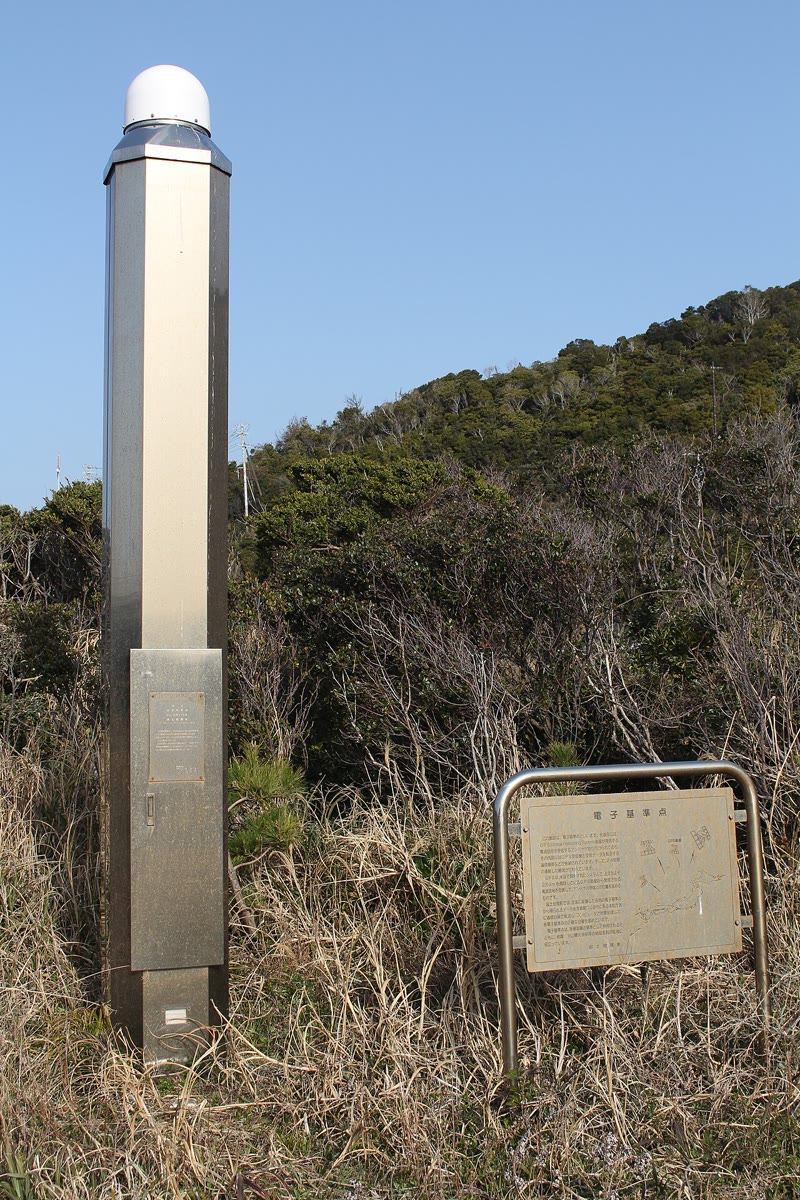
\includegraphics[width=\linewidth]{images/book3/b1-gnss-station.jpg}

{\scriptsize Stasiun permanen di Jepang, antenanya di bawah kubah (Alpsdake, CC BY-SA 4.0).}
\end{minipage}
\end{inthefield}

Kecepatan stasiun di bagian dalam dua lempeng memberikan \omterm{def:b1:plate-kinematics:euler-pole}{vektor Euler} sendiri, tidak bergantung pada catatan geologi. Untuk Eurasia relatif terhadap Amerika Utara, vektor seperti itu memprediksi \qty{17.0}{mm.yr^{-1}} di Islandia, sekitar \qty{8}{\percent} lebih sedikit daripada \qty{18.6}{mm.yr^{-1}} yang dirata-ratakan selama \qty{3.16}{Ma} (gambar di atas). Garis di antara Reykjavik dan Stavanger, keduanya di bagian \omterm{def:b1:plate-kinematics:triple-junction}{stabil} lempengnya, bertambah \qty{17.5}{mm.yr^{-1}}; vektor satelit memprediksi \qty{17.1}{mm.yr^{-1}}, vektor geologi \qty{18.6}{mm.yr^{-1}}. Di seluruh Atlantik Utara, laju yang diukur selama beberapa dekade dan laju yang dirata-ratakan selama tiga juta tahun karena itu sepakat hingga sepersepuluh: di sana lempeng-lempeng bergerak hari ini hampir seperti yang telah mereka lakukan selama jutaan tahun.
% ledger: morvel:gps-eu-na, morvel:eu-na, ngl:reyk, ngl:stas (chord rates computed in calc/ch12.py)

Di dalam zona batas gambarannya kurang sederhana, karena stasiun bergerak lebih daripada lempeng-lempengnya. Lebih dari sepersepuluh Islandia berada di bawah tudung es, dan sebagian besar darinya telah kehilangan massa sejak sekitar 1890: \omterm{def:b1:layered-earth:layers}{kerak} di bawahnya naik ketika beban berkurang, dan bergerak mendatar menjauhi es yang menipis. Stasiun di Höfn, di pantai tenggara dekat tudung es terbesar, naik sebesar \qty{12.9}{mm.yr^{-1}}.
% ledger: spaans:iceland-gia, ngl:hofn

\section{Latihan}

Ambil $R = \qty{6371}{km}$ di seluruh bagian.

\begin{exercise}[$\star$]\label{exo:b1:plate-kinematics:1}
\omterm{def:b1:plate-kinematics:euler-pole}{Vektor Euler} Eurasia relatif terhadap Amerika Utara memiliki laju \qty{0.210}{\degree\per\Ma}. (a) Ubah ke \unit{rad.yr^{-1}} dan ke \unit{rad.s^{-1}}. (b) Berapa lama satu putaran penuh? (c) Hitung $\omega R$ dalam \unit{mm.yr^{-1}}.
% ledger: morvel:eu-na
\end{exercise}

\begin{exercise}[$\star$]\label{exo:b1:plate-kinematics:2}
Dengan \omterm{def:b1:plate-kinematics:euler-pole}{vektor Euler} yang sama, hitung kelajuan relatif kedua lempeng pada \ang{30}, \ang{60} dan \ang{90} dari \omterm{def:b1:plate-kinematics:euler-pole}{kutub Euler}. Di mana sepanjang batas lempeng penyebaran paling cepat?
\end{exercise}

\begin{exercise}[$\star$]\label{exo:b1:plate-kinematics:3}
Subkron normal Jaramillo berlangsung dari \qty{1.072}{Ma} hingga \qty{0.988}{Ma}. (a) Seberapa lebar pita yang dibuatnya di setiap sisi punggungan dengan \omterm{def:b1:plate-kinematics:spreading-rate}{laju penyebaran setengah} \qty{50}{mm.yr^{-1}}? Dengan \qty{10}{mm.yr^{-1}}? (b) Berapa lebar total pita kron normal sekarang, yang dimulai \qty{0.781}{Ma}, di punggungan dengan laju setengah \qty{10}{mm.yr^{-1}}?
% ledger: iodp:gpts2004
\end{exercise}

\begin{exercise}[$\star$]\label{exo:b1:plate-kinematics:4}
Pada suatu profil melintasi sebuah punggungan, tepi muda anomali kron C2An, berumur \qty{2.581}{Ma}, berada \qty{66}{km} di barat sumbu dan \qty{64}{km} di timur. Hitung dua laju setengah penyebaran dan \omterm{def:b1:plate-kinematics:spreading-rate}{laju penyebaran penuh}. Apakah penyebarannya simetris?
% ledger: iodp:gpts2004
\end{exercise}

\begin{exercise}[$\star\star$]\label{exo:b1:plate-kinematics:5}
Sebuah titik di Punggungan Gakkel, di Samudra Arktik, berada pada \ang{85}\,U, \ang{0}\,T. Hitung jarak sudutnya dari \omterm{def:b1:plate-kinematics:euler-pole}{kutub Euler} Eurasia--Amerika Utara (\ang{61.8}\,U, \ang{139.6}\,T, \qty{0.210}{\degree\per\Ma}) dan laju penyebarannya di sana. Bandingkan dengan laju terukur \qtyrange{11}{12}{mm.yr^{-1}}.
% ledger: morvel:eu-na
\end{exercise}

\begin{exercise}[$\star\star$]\label{exo:b1:plate-kinematics:6}
Pada \omterm{def:b1:plate-kinematics:triple-junction}{titik tiga} Azores, \ang{39.44}\,U, \ang{29.83}\,B, hitung (a) jarak sudut ke \omterm{def:b1:plate-kinematics:euler-pole}{kutub Euler} Eurasia--Amerika Utara, (b) laju penyebaran, dan (c) \omterm{def:b1:spherical-astronomy:horizontal}{azimut} gerak relatif. (d) \omterm{def:b1:field-lab-methods-1:trend-plunge}{Trend} apa yang Anda prediksikan untuk sesar transform punggungan tepat di utara titik itu?
% ledger: morvel:eu-na, morvel:azores
\end{exercise}

\begin{exercise}[$\star\star$]\label{exo:b1:plate-kinematics:7}
(a) Tuliskan \omterm{def:b1:plate-kinematics:euler-pole}{vektor Euler} $\vec\omega_{\mathrm{EU\,NA}}$ (\ang{61.8}\,U, \ang{139.6}\,T, \qty{0.210}{\degree\per\Ma}) dan $\vec\omega_{\mathrm{NB\,NA}}$ (\ang{79.2}\,U, \ang{40.2}\,T, \qty{0.233}{\degree\per\Ma}) dalam komponen Kartesius, dalam \unit{\degree\per\Ma}. (b) Turunkan $\vec\omega_{\mathrm{NB\,EU}}$, kutub dan lajunya. (c) Mengapa ini cara terbaik untuk mengetahui gerak Nubia relatif terhadap Eurasia?
% ledger: morvel:eu-na, morvel:nb-na
\end{exercise}

\begin{exercise}[$\star\star$]\label{exo:b1:plate-kinematics:8}
Misalkan $\vec e_x$ menunjuk ke \ang{0}\,U, \ang{0}\,T, $\vec e_y$ ke \ang{0}\,U, \ang{90}\,T dan $\vec e_z$ ke kutub utara. Dengan rumus Rodrigues, hitung bayangan $\vec e_x$ (a) oleh rotasi \ang{90} terhadap $\vec e_z$ diikuti rotasi \ang{90} terhadap $\vec e_x$; (b) oleh dua rotasi yang sama dalam urutan sebaliknya. (c) Apa artinya ini bagi rekonstruksi posisi lempeng di masa lalu?
\end{exercise}

\begin{exercise}[$\star\star$]\label{exo:b1:plate-kinematics:9}
Tiga lempeng A, B dan C bertemu pada sebuah \omterm{def:b1:plate-kinematics:triple-junction}{titik tiga} punggungan--punggungan--punggungan. Relatif terhadap A, lempeng B bergerak sebesar \qty{30}{mm.yr^{-1}} menuju timur dan lempeng C sebesar \qty{40}{mm.yr^{-1}} menuju selatan. (a) Gambarkan segitiga kecepatannya. (b) Hitung kelajuan dan \omterm{def:b1:spherical-astronomy:horizontal}{azimut} C relatif terhadap B. (c) Berapa \omterm{def:b1:field-lab-methods-1:trend-plunge}{trend} punggungan antara B dan C jika ia menyebar tegak lurus terhadap sumbunya?
\end{exercise}

\begin{exercise}[$\star\star\star$]\label{exo:b1:plate-kinematics:10}
(a) Tunjukkan bahwa jejak matriks $R$ dari rotasi sebesar $\alpha$ terhadap sumbu mana pun
adalah $1 + 2\cos\alpha$. (b) Matriks
\[
  R = \begin{pmatrix} 0 & 0 & 1\\ 1 & 0 & 0\\ 0 & 1 & 0\end{pmatrix}
\]
adalah ortogonal dengan determinan $1$. Cari sumbunya, sebagai \omterm{def:b1:spherical-astronomy:geographic}{lintang} dan \omterm{def:b1:spherical-astronomy:geographic}{bujur}, dan sudutnya. (c) Periksa jawaban Anda dengan menerapkan $R$ pada $\vec e_x$, $\vec e_y$
dan $\vec e_z$.
\end{exercise}

\begin{exercise}[$\star\star\star$]\label{exo:b1:plate-kinematics:11}
Sebelum penentuan posisi satelit, \omterm{def:b1:plate-kinematics:euler-pole}{kutub Euler} ditemukan dari arah sesar transform. (a) Tunjukkan bahwa \omterm{def:b1:plate-kinematics:euler-pole}{kutub Euler} berada pada \omterm{def:b1:spherical-astronomy:spherical-triangle}{lingkaran besar} yang melalui sebuah titik sesar transform dan tegak lurus terhadap sesar di sana, dan bahwa kutub itu karena itu berada sepanjang $\vec t_1\times\vec t_2$, dengan $\vec t_1$ dan $\vec t_2$ vektor satuan sepanjang dua sesar transform dari batas yang sama.
(b) Sesar transform membentang pada \ang{95} di dekat \omterm{def:b1:plate-kinematics:triple-junction}{titik tiga} Azores
(\ang{39.44}\,U, \ang{29.83}\,B) dan pada \ang{103} di Islandia (\ang{64.5}\,U,
\ang{18}\,B). Vektor satuan horizontal pada \omterm{def:b1:spherical-astronomy:geographic}{lintang} $\varphi$ dan \omterm{def:b1:spherical-astronomy:geographic}{bujur}
$\lambda$ yang menunjuk ke \omterm{def:b1:spherical-astronomy:horizontal}{azimut} $\beta$ adalah $\sin\beta\,\vec e +
\cos\beta\,\vec n$, dengan $\vec e = (-\sin\lambda, \cos\lambda, 0)$ dan $\vec n =
(-\sin\varphi\cos\lambda, -\sin\varphi\sin\lambda, \cos\varphi)$. Tentukan
kutubnya. (c) Seberapa baik dua transform menentukan kutub?
% ledger: morvel:eu-na
\end{exercise}

\begin{exercise}[$\star\star\star$]\label{exo:b1:plate-kinematics:12}
Posisi timur sebuah stasiun, setiap tiga bulan selama tiga tahun, adalah
(dalam milimeter, dari $t = 0$):
\begin{center}\small
\begin{tabular}{l*{13}{c}}
\hline
$t$ (yr) & 0 & 0.25 & 0.5 & 0.75 & 1 & 1.25 & 1.5 & 1.75 & 2 & 2.25 & 2.5 & 2.75 & 3\\
$x$ (mm) & 4 & 5 & 6 & 15 & 24 & 25 & 26 & 65 & 74 & 75 & 76 & 85 & 94\\
\hline
\end{tabular}
\end{center}
Deret ini terdiri atas gerak yang mantap, osilasi musiman dan lompatan yang disebabkan oleh gempa. (a) Hitung kecepatan dari posisi pertama dan terakhir. (b) Hitung sembilan selisih antara posisi yang berjarak tepat satu tahun, dan median-nya. (c) Jelaskan mengapa median selisih satu tahunan adalah perkiraan yang tangguh untuk kecepatan mantap, dan kapan ia akan gagal.
\end{exercise}

\section{Soal: Islandia terbelah}

\begin{problem}[{Soal akhir pekan --- pembukaan Atlantik Utara di seluruh Islandia, diukur dengan tiga cara}]
\label{pb:b1:plate-kinematics:1}
% values: calc/ch12.py (Part II profile invented for the problem; real Euler
% vectors, chron ages and station velocities)
% ledger: morvel:eu-na, morvel:nb-na, iodp:gpts2004, ngl:reyk, ngl:stas, ngl:hofn
Islandia terletak di atas Punggungan Atlantik Tengah, di antara lempeng Amerika Utara di barat dan lempeng Eurasia di timur. Ambil $R = \qty{6371}{km}$ dan, untuk Eurasia relatif terhadap Amerika Utara, \omterm{def:b1:plate-kinematics:euler-pole}{vektor Euler} dengan kutubnya pada \ang{61.8}\,U, \ang{139.6}\,T dan laju \qty{0.210}{\degree\per\Ma}.

\medskip
\noindent\textbf{Bagian I --- Vektor lempeng.}
\begin{enumerate}
  \item Ubah laju ke \unit{rad.yr^{-1}} dan hitung $\omega R$ dalam \unit{mm.yr^{-1}}.
  \item Hitung jarak sudut $\Delta$ dari kutub ke pusat Islandia, \ang{64.5}\,U, \ang{18}\,B.
  \item Turunkan \omterm{def:b1:plate-kinematics:spreading-rate}{laju penyebaran penuh} di seluruh Islandia yang diprediksi oleh vektor lempeng.
  \item Hitung \omterm{def:b1:spherical-astronomy:horizontal}{azimut} kutub yang dilihat dari Islandia, dan \omterm{def:b1:spherical-astronomy:horizontal}{azimut} gerak Eurasia relatif terhadap Amerika Utara.
  \item Uraikan kecepatan ini menjadi komponen timur dan utara.
  \item Di Punggungan Gakkel, pada \ang{86}\,U, \ang{60}\,T, laju apa yang diberikan vektor yang sama? Mengapa batas di sana jauh lebih lambat?
\end{enumerate}

\noindent\textbf{Bagian II --- Pita magnetik.}
Sebuah profil magnetik kapal melintasi Punggungan Reykjanes, di barat daya Islandia dekat \ang{63}\,U, \ang{23}\,B, dijalankan searah penyebaran, memberikan jarak berikut dari sumbu ke tiga batas kron (profil yang disusun untuk soal ini):
\begin{center}\small
\begin{tabular}{lccc}
\hline
batas & umur (Ma) & barat sumbu (km) & timur sumbu (km)\\
\hline
dasar C1n & 0.781 & 9.7 & 10.1\\
tepi muda C2An & 2.581 & 26.8 & 27.3\\
tepi muda C5n & 9.779 & 94 & 97\\
\hline
\end{tabular}
\end{center}
\begin{enumerate}[resume]
  \item Dari tepi muda C5n, hitung dua \omterm{def:b1:plate-kinematics:spreading-rate}{laju penyebaran setengah}.
  \item Turunkan \omterm{def:b1:plate-kinematics:spreading-rate}{laju penyebaran penuh} sejak \qty{9.8}{Ma}.
  \item Hitung juga laju penuh dari dua batas yang lebih muda. Apakah ketiganya sepakat? Jelaskan bagaimana mereka berubah dengan umur batas.
  \item Apakah penyebarannya simetris? Apakah asimetri itu mengubah laju penuh?
  \item Di Punggungan Reykjanes, batas antara pita tergeser menjauhi sumbu sebesar \qty{5.0}{km} secara keseluruhan, kedua sisi bersama-sama. Koreksi ketiga laju penuh. Mengapa koreksi itu paling berpengaruh pada batas yang termuda?
  \item Berapa lebar pita subkron Jaramillo (\qtyrange{1.072}{0.988}{Ma}) di setiap sisi, pada laju setengah yang terkoreksi? Bandingkan dengan pergeseran pada soal 11. Anomali Jaramillo tetap dikenali dengan jelas pada profil Punggungan Reykjanes, tetapi tidak ada di Punggungan Gakkel: apa yang disarankan oleh itu?
  \item Vektor lempeng memprediksi \qty{19.0}{mm.yr^{-1}} di profil itu. Bandingkan dengan laju-laju terkoreksi Anda.
\end{enumerate}

\noindent\textbf{Bagian III --- Satelit.}
Stasiun permanen REYK (Reykjavik, \ang{64.139}\,U, \ang{21.955}\,B) dan STAS (Stavanger, \ang{59.018}\,U, \ang{5.599}\,T) terletak di lempeng Amerika Utara dan Eurasia. Kecepatan terukur mereka membuat garis di antara keduanya bertambah sebesar \qty{17.5}{mm.yr^{-1}}.
\begin{enumerate}[resume]
  \item Hitung jarak sudut antara kedua stasiun, dan panjang garis lurusnya.
  \item Berapa lama garis itu memerlukan waktu untuk bertambah satu meter?
  \item Vektor lempeng memberi STAS kecepatan \qty{18.9}{mm.yr^{-1}} menuju \ang{114.8} relatif terhadap Amerika Utara. \omterm{def:b1:spherical-astronomy:spherical-triangle}{Lingkaran besar} dari REYK tiba di STAS dengan arah menuju \ang{123.1}. Hitung komponen kecepatan sepanjang arah ini, lalu pertambahan garis yang diprediksi, yang membentuk sudut $\Delta/2$ dengan horizontal di STAS.
  \item Bandingkan pertambahan yang terukur dan yang diprediksi. Apa yang mungkin menjelaskan selisihnya?
  \item Relatif terhadap Amerika Utara, REYK bergerak sebesar \qty{1.07}{mm.yr^{-1}} ke barat dan \qty{0.97}{mm.yr^{-1}} ke selatan, dan stasiun HOFN (Höfn, Islandia tenggara) sebesar \qty{21.12}{mm.yr^{-1}} ke timur dan \qty{6.97}{mm.yr^{-1}} ke selatan. Hitung kelajuan dan \omterm{def:b1:spherical-astronomy:horizontal}{azimut} HOFN relatif terhadap REYK.
  \item Bandingkan dengan Bagian I. HOFN juga naik sebesar \qty{12.9}{mm.yr^{-1}}. Mengapa stasiun di dalam Islandia adalah ukuran gerak lempeng yang buruk?
\end{enumerate}

\noindent\textbf{Bagian IV --- Sepuluh juta tahun, dan titik tiga di selatan.}
\begin{enumerate}[resume]
  \item Selama \qty{10}{Ma}, melalui sudut berapa Eurasia berputar relatif terhadap Amerika Utara terhadap kutub?
  \item Sejauh mana sebuah titik Eurasia di tengah Islandia menempuh \omterm{def:b1:spherical-astronomy:spherical-triangle}{lingkaran kecilnya} dalam waktu itu? Bandingkan dengan lebar \omterm{def:b1:layered-earth:layers}{kerak} yang terkoreksi, yang terbentuk sejak tepi muda C5n dalam Bagian II.
  \item Di \omterm{def:b1:plate-kinematics:triple-junction}{titik tiga} Azores, vektor lempeng memberikan Eurasia \qty{22.9}{mm.yr^{-1}} menuju \ang{95.1} dan Nubia \qty{19.2}{mm.yr^{-1}} menuju \ang{103.8}, keduanya relatif terhadap Amerika Utara. Hitung kecepatan Eurasia relatif terhadap Nubia.
  \item Apakah \omterm{def:b1:plate-kinematics:triple-junction}{titik tiga} ini \omterm{def:b1:plate-kinematics:triple-junction}{stabil}? Jenis batas apa yang diimplikasikan oleh kecepatan pada soal 22 antara Eurasia dan Nubia?
  \item Kumpulkan laju pembukaan dari Bagian I, II dan III. Mana yang sepakat, dan metode mana yang mengukur gerak lempeng dalam waktu terpendek?
  \item Hingga milimeter per tahun terdekat, \omterm{def:b1:plate-kinematics:spreading-rate}{laju penyebaran penuh} di seluruh Islandia apa yang diberikan oleh vektor lempeng dan oleh pita magnetik yang terkoreksi?
\end{enumerate}
\end{problem}
